\chapter{Théorie d'un réseau acoustique de résonateur de Helmholtz fini}
Le but du projet est de caractériser un réseau de résonateur de Helmholtz placés sur un guide d'onde. On dispose pour cela d'un banc de mesure représenté figure ~\ref{schema_infini}. Une simulation de la propagation dans le réseau pourra donc être confronté à une expérience.

\begin{figure}[!ht] \centering
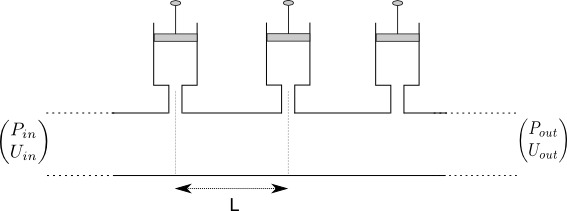
\includegraphics[scale=0.5]{./images_chp1/schema_reseau_infini.png}
\caption{\label{schema_infini} Schéma du réseau de résonateurs de Helmholtz.}
\end{figure}


\section{Mise sous forme matricielle}
On s’intéresse ici a la mise sous forme matricielle du problème de la propagation acoustique dans le réseau periodique vu ci-dessus. Le but étant de mettre le système sous la forme suivante:
\begin{equation}
\begin{pmatrix} P_{out} \\ U_{out} \end{pmatrix} =\begin{pmatrix} A & B \\ C & D \end{pmatrix}^N \begin{pmatrix} P_{in} \\ U_{in} \end{pmatrix} 
\end{equation}

Cette matrice dispose en effet de propriétés intéressantes et l'étude du système sera grandement facilité par ce formalise.

Pour cela, les 2 éléments du réseau (guide et résonateur) doivent être mis sous forme matricielle puis multipliés.

\subsection{Le guide d'onde}
La solution de la propagation dans un guide d'onde peux être facilement déduite de l'équation d'onde suivante:
\begin{equation}
\frac{\partial ^2 p}{\partial x^2} -\frac{1}{c^{2}} \frac{\partial ^2 p}{\partial t^2}= 0
\end{equation}

On se place en régime harmonique et on note $\Gamma = jk$ la constante de propagation du système. D’où les solutions (vitesses calculées avec l'équation d'Euler:

\begin{eqnarray*}
\begin{cases}
p(x_1)  =  A e^{-\Gamma x_1} + B e^{\Gamma x_1} \\
v(x_1)  =  -\frac{1}{j\omega\rho} [ -\Gamma A e^{-\Gamma x_1} + \Gamma e^{\Gamma x_1}]\\
p(x_2)  =  A e^{-\Gamma x_2} + B e^{\Gamma x_2} \\
v(x_2)  =  -\frac{1}{j\omega\rho} [ -\Gamma A e^{-\Gamma x_2} + \Gamma e^{\Gamma x_2}]
\end{cases}
\end{eqnarray*}
 
On pose $x_1 - x_2 = L$. Tous calculs faits, on trouve finalement:
\begin{eqnarray*}
\begin{pmatrix} p(x_1) \\ v(x_1) \end{pmatrix} = \begin{pmatrix} \cosh(kL) & \frac{j\omega\rho}{k} \sinh(k L) \\  \frac{k}{j\omega\rho}\sinh(k L) & \cosh(k L) \end{pmatrix} \begin{pmatrix} p(x_2) \\ v(x_2) \end{pmatrix}
\end{eqnarray*}


%Cas sans pertes ($\Gamma = j k = jw/c$):
%\begin{eqnarray*}
%\begin{pmatrix} p(x_1) \\ v(x_1) \end{pmatrix} = \begin{pmatrix} \cos(k L) & j Z_c \sin(k L) \\ \frac{1}{Z_c} \sin(k L) & \cos(k L) \end{pmatrix} \begin{pmatrix} p(x_2)\\ v(x_2) \end{pmatrix}
%\end{eqnarray*}
%Avec $Z_c = \frac{\rho c}{S}$ où $S$ est la section du tube.

\subsubsection{Ajout des pertes}

Pour prendre en compte les pertes, on modifie l'expression de la constante de propagation et de l'impédance caractéristique. Les expressions utilisées se trouvent en [A1]. on a donc:
\begin{eqnarray*}
 k =  \frac{\omega}{c_0} \left( 1 + \frac{\beta}{s}(1+(\gamma-1)/ \chi \right) \\
 Z_c =  \frac{\rho c_0}{S} \left( 1 + \frac{\beta}{s}(1-(\gamma-1)/ \chi \right) 
\end{eqnarray*}

Et où on a:
\begin{itemize}
 \item  $s=R/ \delta$ avec $\delta = \sqrt{\frac{2 \mu}{\rho \omega}}$
 \item  $\chi = \sqrt{P_r}$ ou $P_r$ est le nombre de Prandtl
 \item $\beta = (1-j)/\sqrt{2}$ 
 \item $\mu$ la viscosité de l'air
\end{itemize}



\subsection{Le résonateur}
Le résonateur est considéré dans le réseau comme un changement ponctuel d'impédance.

On a la formule de l'impédance ramenée suivante:
\begin{eqnarray}
Z{x_1}=\frac{jZ_c tan(kL)+Z_{x_2}}{1+j\frac{Z_{x_2}}{Z_c}tan(kL)}.
\end{eqnarray}

Si on suppose que le résonateur est constitué d'une parois rigide et de 2 tubes, on peux calculer sont impédance comme suit:

\begin{eqnarray*}
\begin{pmatrix} P_2 \\U_2 \end{pmatrix} = \begin{pmatrix} \cos(k l) & j Z_{c_1} \sin(k l) \\ \frac{1}{Z_{c_1}} \sin(k l) & \cos(k l) \end{pmatrix} \begin{pmatrix} \cos(k L) & j Z_{c_2} \sin(k L) \\ \frac{1}{Z_{c_2}} \sin(k L) & \cos(k L) \end{pmatrix} \begin{pmatrix} P_1 \\ 0  \end{pmatrix} \\
\begin{pmatrix} P_2 \\U_2 \end{pmatrix} = \begin{pmatrix} A B \\ C D \end{pmatrix} \begin{pmatrix} P_1 \\ 0  \end{pmatrix} \\
\Leftrightarrow Z_{resonateur} = \frac{A}{C}
\end{eqnarray*}


Si on ajoute un résonateur en parallèle au guide, on a toujours continuité des pressions mais plus des vitesses. On a donc la matrice de transfert pression-vitesse suivante pour un résonateur dans le réseau:

\begin{eqnarray*}
M_{resonateur} = \begin{pmatrix} 1 &  0 \\ 1 /Z_{resonateur} & 1  \end{pmatrix}\\
\end{eqnarray*}

\section{Étude du réseau fini}

Une fois les matrices de guide et de résonateur connues, il suffit alors de les multiplier afin d'obtenir la matrice d'une cellule du réseau.

\subsection{Équation de dispersion}
\subsection{Bande de Bragg}
\subsection{Bande interdites liés aux résonateurs}
\subsection{Réflexion et transmission du réseau}
